\documentclass{article}

\usepackage[
	top=2cm, 
	bottom=2cm, 
	left=2.5cm, 
	right=2.5cm
]{geometry}
\usepackage{listings}
\lstset{basicstyle=\ttfamily,
  showstringspaces=false,
  commentstyle=\color{red},
  keywordstyle=\color{blue}
}
\usepackage{amsmath}
\usepackage{amsfonts}
\usepackage{fontspec}
\usepackage{xepersian}

\settextfont[Scale=1.1]{XB Niloofar}
\setlatintextfont{Times New Roman}
\baselineskip=6mm
\renewcommand{\baselinestretch}{1.7}
\setlength{\columnsep}{27pt}

\title{پروژه درس بهینه سازی آنلاین}
\author{سید سروش هاشمی (۹۷۲۰۱۱۴۸)}
\date{\today}

\begin{document}
\maketitle

\section{صورت مسئله}
در این مسئله قرار است از روی عکس حروف انگلیسی، حدس بزنیم چه حرفی است. اما ورودی این مسئله عکس نیست بلکه یک مجموعه خط است که نقاط شروع و پایان و طول آن ها به ما داده شده. یعنی به ازای هر عکس، به ما مختصات شروع و پایان خط های موجود در عکس و همچنین مساحت کوچکترین مستطیلی که کل کاراکتر موجود در عکس در آن جا می شود. بنابراین ممکن است به ازای یک عکس ۴ خط و به ازای یک عکس دیگر ۱۰ خط داشته باشیم.

\section{نحوه حل مسئله به کمک یادگیری آنلاین}
از الگوریتم مشاوران برای حل این مسئله استفاده می کنیم. می توانیم تعداد زیادی تابع به صورت تصادفی تولید کنیم و به عنوان مشاوران از آن ها استفاده کنیم. اما با این کار میزان محاسبات الگوریتم آنلاین به شدت زیاد می شود. برای حل این مشکل، باید چند مشاور خوب را اول کار انتخاب کنیم و الگوریتم مشاوران را فقط روی آن ها اجرا کنیم. الگوریتم های مشاوران در این پروژه به شرح زیر است:
\begin{itemize}
\item
رگرسیون خطی
\item
\lr{random forest}
\item
SVM
\item
شبکه عصبی 
\lr{fully connected} 
با سه لایه مخفی با اندازه های ۱۰۰، ۸۰، و ۵۰ نورون
\end{itemize}

ابتدا درصد کوچکی از داده های مسئله را به طور تصادفی انتخاب کردم و این مدل ها را با آن آموزش دادم. سپس الگوریتم 
\lr{Weighted Majority} 
را روی این مشاوران اجرا کردم. می توانید خطای هر یک از مشاوران و خطای الگوریتم آنلاین را در نمودار زیر ببینید. خطای هر یک از مشاوران و الگوریتم آنلاین در مرحله 
$t$ 
برابر صفر است اگر درست حدس زده باشند و برابر ۱ است اگر اشتباه حدس زده باشند. اگر 
$l_t$ 
را مجموع خطا تا مرحله 
$t$ 
بگیریم، نمودار زیر 
$\frac{l_t}{t}$ 
را نشان می دهد. 

\begin{center}
	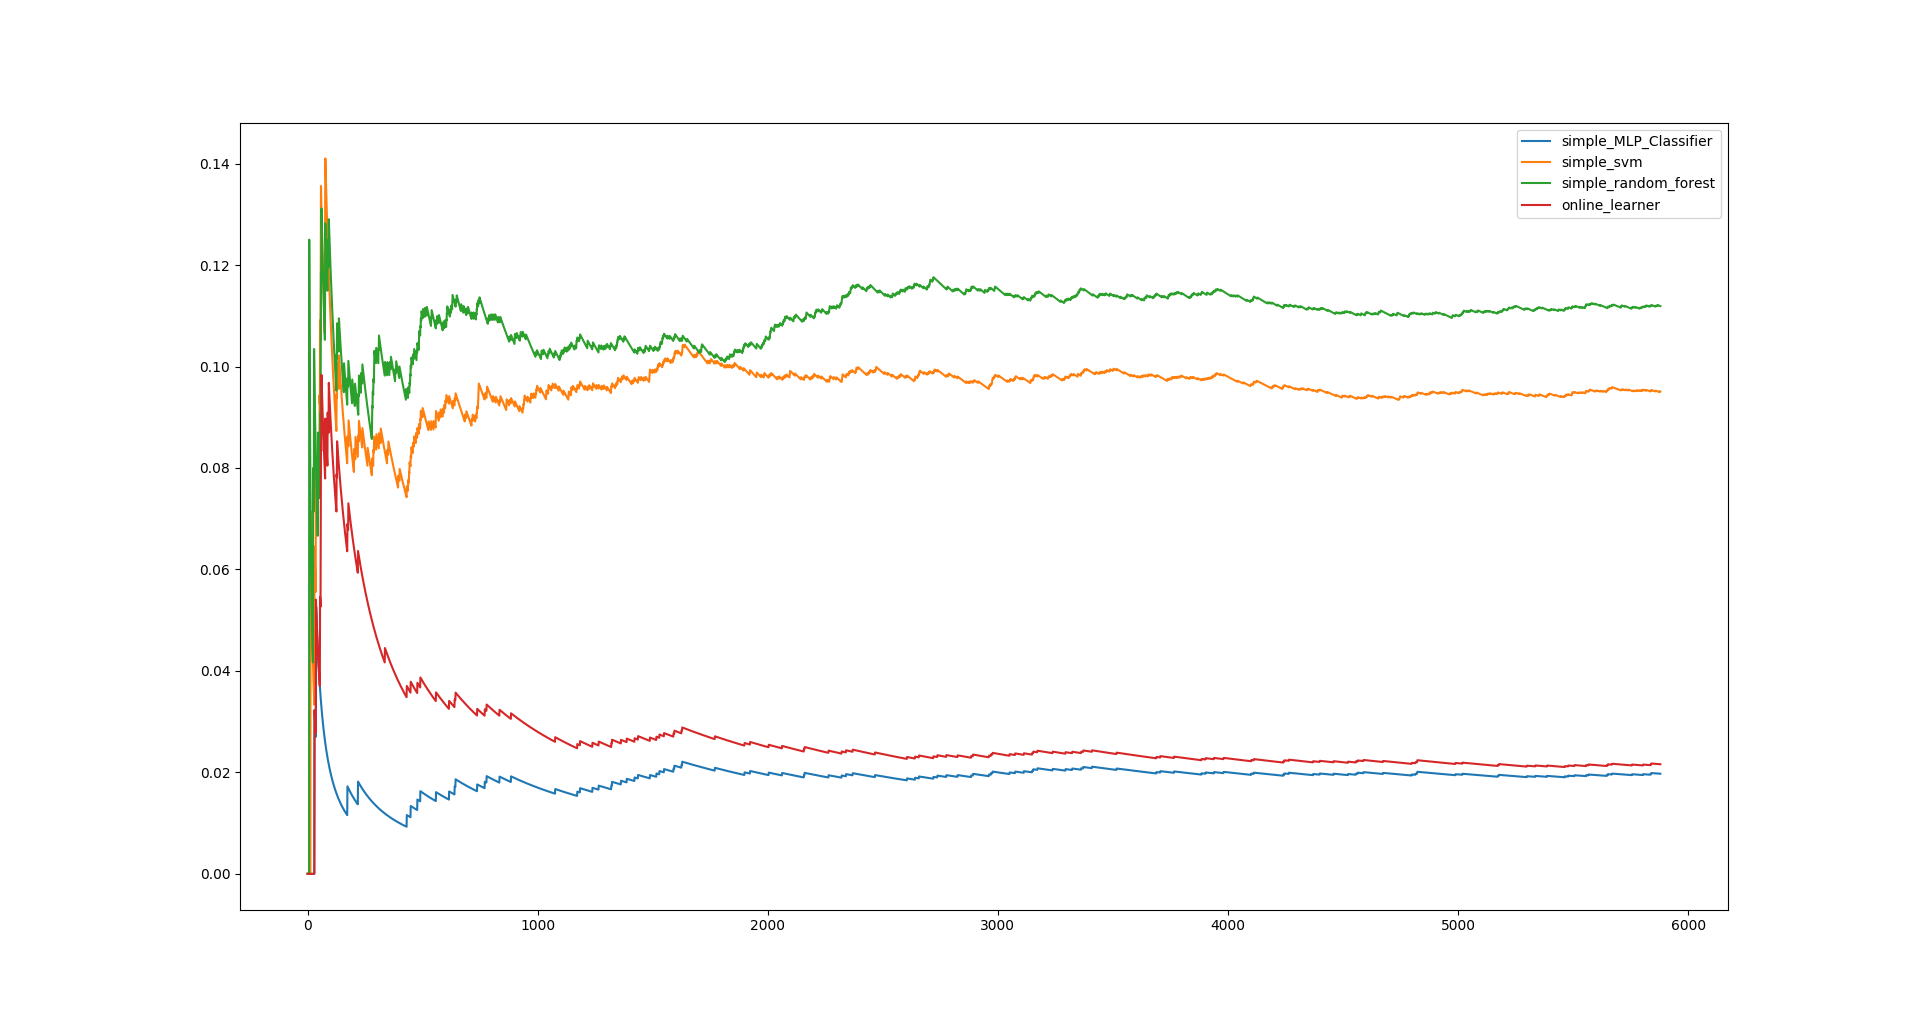
\includegraphics[width=\columnwidth]{loss_t.png}
\end{center}

\section{نحوه اجرای کد}
کد این پروژه با پایتون نوشته شده. برای اجرای آن ابتدا یک 
\lr{virtual environment} 
بسازید و 
\lr{requirements} 
های پروژه را با دستور زیر نصب کنید

\begin{latin}
\begin{lstlisting}[language=bash]
python -m pip install -r requirements.txt
\end{lstlisting}
\end{latin}

سپس می توانید با این دستور داده های مسئله را به صورت تصادفی به دو بخش آنلاین و آفلاین تقسیم کنید. باید به جای علامت سوال بگویید می خواهید چند درصد از داده های اصلی برای مسئله آنلاین استفاده شود. مثلا 0.98 می تواند مقدار خوبی باشد. این دستور داده های آنلاین و آفلاین را با فرمت 
\lr{JSON} 
در فولدر 
\lr{data} 
ذخیره می کند.

\begin{latin}
\begin{lstlisting}[language=bash]
make split_online_offline_datasets online=???
\end{lstlisting}
\end{latin}

حال باید به کمک داده های آفلاین، مشاوران را آموزش دهد. برای این کار دستور زیر را اجرا کنید. این دستور تک تک مشاوران را با این داده آموزش داده و مدل آموزش داده شده را در فولدر 
\lr{trained\_models} 
ذخیره می کند. کد مشاوران در فولدر 
\lr{codes/experts} 
نوشته شده است.

\begin{latin}
\begin{lstlisting}[language=bash]
make train_experts
\end{lstlisting}
\end{latin}

حال همه چیز برای اجرای الگوریتم آنلاین آماده است. دستور زیر را اجرا کنید. این دستور مدل های آموزش دیده شده و ذخیره شده مشاوران را 
\lr{load} 
می کند و الگوریتم 
\lr{Weighted Majority} 
را روی آن ها اجرا می کند.

\begin{latin}
\begin{lstlisting}[language=bash]
make go_online
\end{lstlisting}
\end{latin}

\section{تحلیل مشاهدات}
در نمودار به خوبی مشخص است که الگوریتم آنلاین به سرعت به سمت بهترین مشاور رفته است. به طور دقیق تر از حدود حرکت ۲۰۰ ام، الگوریتم انتخاب مشاور، تقریبا همیشه مشاور شبکه عصبی را انتخاب کرده که بنابر میزان خطای آن، بهترین مشاور است.

\end{document}